\documentclass[../thesis.tex]{subfiles}

\begin{document}

\chapter{Introduction}
\label{chap:intro}

\section{Neutrinos and the Standard Model}
\label{sec:neuAndSM}

The Standard Model (SM) of particle physics~\cite{Rosner_2001zy} has proven to be an enormous success. From a handful of ingredients---three gauge groups, three generations of quarks and leptons, the Higgs field, and 18 free parameters---the SM provides a succinct and precise description of nature that agrees incredibly well with the bulk of experimental observations.

However, even if we ignore the glaring absence of gravity in the theory (a difficulty inherent to quantum field theory itself), there are clear and exciting signs that new physics must lie beyond the Standard Model. For instance, the SM fails to explain dark matter, dark energy, cosmic inflation, the lightness of the electroweak scale, and the matter/antimatter asymmetry of the Universe, among other puzzles.

These are difficult problems which may take decades to resolve, and in most cases there is little clarity on how the SM will need to be extended along the way. On the other hand, the last half-century has produced overwhelming evidence of another Beyond the Standard Model (BSM) effect, one that admits a relatively successful quantitative description: neutrino mixing. Before discussing this phenomenon, it is worthwhile to review the story of the neutrino itself.

More than a century ago, measurements of nuclear beta decay gave the surprising result that the energy of the outgoing electron was continuously distributed~\cite{Chadwick:262756}, in stark contrast to the discrete lines observed in alpha and gamma decay. If, like alpha and gamma decay, beta decay were a two-body process, then a continuous spectrum would seem to imply the violation of energy and momentum conservation. Furthermore, it had been observed that nuclear spin is either integral (for even mass numbers) or half-integral (for odd mass numbers), implying that the nuclear spin can only change by an integer during beta decays, which conserve the mass number. And yet, the electron has a spin of 1/2, so a two-body process would also imply the nonconservation of angular momentum. Did all of this mean that, alas, it was necessary to discard the most sacred conservation laws of physics?

An alternative resolution, one that would avoid violations of the conservation laws, was proposed in 1930 by Pauli, who postulated the existence of a yet-unobserved, light, neutral particle, or ``neutron'', contained in the nucleus and emitted along with the electron in beta decay~\cite{Pauli:83282}. Chadwick's 1932 discovery of the actual neutron led Fermi and others to redub Pauli's hypothetical particle as the \emph{neutrino}. In 1933, Fermi's theory of beta decay~\cite{Fermi1934TentativoDU}, which incorporated the neutrino, was successful in reproducing the measured electron spectra, but the neutrino itself would not be directly observed for another two decades.

In 1956, antineutrinos from a nuclear reactor were detected by the Cowan-Reines experiment, marking the first direct confirmation of the neutrino's existence~\cite{Cowan103}. Over the decades that followed, it was found that neutrinos come in three distinct ``flavors''---electron, muon, and tau, corresponding to their charged lepton partners---and that neutrinos lack any discernable mass. These qualities would eventually be incorporated into the Standard Model, which crystallized in the 1970s after a period of remarkable theoretical and experimental progress in particle physics.

Since neutrinos have only ever been observed via their weak interactions, which solely involve the left-handed neutrino state, there is no direct experimental evidence for a right-handed neutrino. Additionally, the observed kinematics of beta decay are, within experimental limits, consistent with the neutrino being massless. Accordingly, in the SM, the three neutrinos are massless left-handed Weyl spinors that interact via the W and Z bosons. From a theoretical standpoint, masslessness is appealing, as it avoids the need to imbue the theory with right-handed neutrinos (which have never been observed) or Majorana mass terms (which are not present for any other SM particle); in addition, since beta decay observations indicate that the neutrino mass must be \emph{very small} if it is nonzero, masslessness avoids the need to explain such unnatural smallness in comparison with the other particles of the theory. Although some puzzling neutrino observations, discussed in \ref{sec:history}, had been known since the late 1960s, massive neutrinos were seldom given serious consideration as the explanation. But as experimental evidence continued to mount, this wall would eventually have to crumble, leading to the revolution that has transpired over the last few decades. Before detailing this history, we provide an overview of the underlying physics, the parameters of which will be referred to repeatedly in our historical discussion.


\section{Neutrino oscillation physics}
\label{sec:oscPhysics}

Neutrino oscillations are the consequence of two facts: First, that the flavor eigenstates are not the same as the mass eigenstates (\emph{mixing}), and second, that the mass eigenvalues aren't fully degenerate (implying that at least one is nonzero). As a result, a flavor eigenstate is a superposition of mass eigenstates which each undergo phase rotation at their own rates; the mass components thus interfere to produce different flavor compositions over time, leading to the observation of oscillations.

The neutrino fields in the flavor and mass bases are related by the Pontecorvo-Maki-Nakagawa-Sakata (PMNS) mixing matrix, $\upmns$ (or simply $U$):
\begin{equation}
  \nu_\alpha = U_{\alpha i} \nu_i,
\end{equation}
that is, for three generations,
\begin{equation}
  \flavcol = \underbrace{\upmnsSimple}_{\upmns} \masscol.
\end{equation}
It can then be shown that the \emph{states} (as opposed to the fields) are related by the complex conjugate of $U$:
\begin{equation}
  \label{eq:nuStateRel}
  \ket{\nu_\alpha} = U^*_{\alpha i}\ket{\nu_i}.
\end{equation}
$\upmns$ can be parameterized in terms of the three mixing angles, $\tAB$, $\tBC$, and $\tAC$, along with a CP-violating complex phase $\dcp$:\footnote{Although a general 3x3 unitary matrix includes six complex phases, most of the phases in a 3x3 \emph{mixing} matrix are physically meaningless. If the neutrinos are Dirac particles, with distinct particle and antiparticle fields, then five of the phases can be absorbed into the definitions of the fields, leaving only one physical phase. It could be inserted anywhere in the factorization of $U$ as long as unitary is preserved, but by convention the definition in \eqref{eq:upmnsParam} is what is used. Conversely, if the neutrinos are Majorana particles, where $\nu = \nubar$ (as discussed in \autoref{sec:majorana}), only three phases can be absorbed, leaving two physical \emph{Majorana phases} in addition to $\dcp$.}
\begin{align}
  \label{eq:upmnsParam}
  \begin{split}
    U &= \upmnsFactored \\\\
    &= \upmnsFull.
  \end{split}
\end{align}
where \(c_{12} \equiv \cos\theta_{12}\) and \(s_{12} \equiv \sin\theta_{12}\), etc. It is these mixing angles (or trigonometric functions thereof), and not the matrix elements themselves, that are directly measured by experiments.

Physically speaking, neutrinos are produced in local processes that conserve energy and momentum. A fully microscopic treatment of neutrino oscillation would therefore require accounting for the neutrino's energy-momentum spread and its entanglement with the other interaction products (as required for energy-momentum conservation). However, for a bulk flux of neutrinos from a known source, the oscillation probability can be derived by simply considering a spacetime-filling plane wave of well-defined energy \emph{or} momentum (but not both). For the physical systems of interest in neutrino oscillation experiments, this approach gives results that agree (for all intents and purposes) with those of a fully self-consistent theoretical treatment \cite{Ligeti}. Indeed, when Daya Bay's data is fit to models that treat the neutrino as a wave packet, the results are completely consistent with the plane-wave approach \cite{DayaBayWavePacket}. As such, for the purposes of this illustrative derivation, we proceed with the plane-wave model.

To calculate the oscillation probability over baseline $L$ for a neutrino of energy
%\footnote{Again, neutrinos are never produced with a well-defined energy, but we ignore this subtlety in what follows, given that the final result remains correct for experiments like Daya Bay.}
% \footnote{In reality, neutrinos are never produced with a well-defined energy, both due to the localization of the production process, and the entanglement of the neutrino with the other products of the interaction (in order to satisfy energy-momentum conservation). A fully self-consistent treatment can be found in \cite{Ligeti}, which confirms that the approximations here nevertheless produce the correct answer, to leading-order, for realistic neutrino oscillation experiments.}
$E$ and initial flavor $\alpha$, we roughly follow\footnote{The derivation in \cite{Giunti_2007} begins with a neutrino of well-defined \emph{momentum} rather than energy. To leading order, the results are the same whether we fix the energy, momentum, or even the velocity. Throughout this work, energy is the variable of interest, so for clarity we choose it to be the fixed quantity here.} \cite{Giunti_2007} and consider a neutrino state $\ket{\nu(x)}$ defined such that:\footnote{In what follows, flavor indices are represented by Greek letters, while mass indices use Roman letters. Also, without loss of generality, we consider only one spatial dimension in this treatment. Time-dependence is ignored, since we are working with an energy eigenstate.}
\begin{equation}
  \ket{\nu(0)} = \ket{\nu_\alpha}.
\end{equation}
That is, at the origin, $\ket{\nu}$ is a flavor eigenstate, consisting of a mixture of mass eigenstates:
\begin{equation}
  \ket{\nu(0)} = U^*_{\alpha i}\ket{\nu_i}.
\end{equation}
The spatial dependence of $\ket{\nu(x)}$ is determined by the fact that the state has a fixed energy $E$. Each mass-eigenstate component $i$ of $\ket{\nu(x)}$ is then a plane wave with momentum
\begin{equation}
  \label{eq:nuStateMomentum}
  p_i = \sqrt{E^2 - m_i^2} = E - \frac{m_i^2}{2E} - \mathcal{O}\left( \frac{m_i^4}{E^3} \right).
\end{equation}
Here, we assume that the masses are very small, below an eV$^2$, which at the $\mathcal{O}$(MeV) energy scales we consider, implies that the higher-order terms in \autoref{eq:nuStateMomentum} are negligible.\footnote{In the case of the electron neutrino, this smallness was obvious from the earliest observations of beta decay kinematics. For the muon neutrino, direct measurements of pion decay \cite{BOOTH196739} provided a less-stringent upper limit on the mass of $\mathcal{O}$(1~MeV), but later oscillation measurements of the mass-squared splittings showed that all three eigenstates indeed possess similarly tiny masses.} We then have
\begin{equation}
  \begin{aligned}
    \label{eq:nuStateSpacetimeDep}
    \ket{\nu(x)} &= e^{ipx} U^*_{\alpha i}\ket{\nu_i} \\
    &\approx \exp \left( i\left[E - \frac{m_i^2}{2E} \right] x \right) U^*_{\alpha i}\ket{\nu_i} \\
    &= \exp \left( iEx - i\frac{m_i^2}{2E}x \right) U^*_{\alpha i}\ket{\nu_i}.
  \end{aligned}
\end{equation}
The common phase factor $e^{iEx}$ has no bearing on the flavor composition of the state, so we drop it, after which \autoref{eq:nuStateSpacetimeDep} simplifies to
\begin{equation}
  \ket{\nu(x)} \approx \exp \left( - i \frac{m_i^2 x}{2E} \right) U^*_{\alpha i} \ket{\nu_i}.
\end{equation}

% This is the point where the limitations of the plane-wave approach become apparent. In reality, neutrinos are not plane waves; they are produced from physically-localized interactions. We have not proven that this model accurately represents the case of a physically-localized state (which would consist of a superposition of plane waves). A wave-packet treatment would allow for a more rigorous physical definition of a propagating neutrino state, but at the expense of requiring assumptions to be made about the initial spatial wavefunction. In any case, it can be shown that, for all reasonable definitions of this initial wavefunction, the oscillation probability very closely agrees with that of the plane-wave approximation \cite{DayaBayWavePacket}

\begin{comment}
To calculate the oscillation probability over baseline $L$ for a neutrino of energy $E$ and initial flavor $\alpha$, we first redefine the problem slightly and consider a neutrino plane wave $\ket{\nu(t)}$ of initial flavor $\alpha$ and well-defined \emph{momentum} $\vec{p}$, such that \(E = |\vec{p}|\).\footnote{One could instead assume a well-defined \emph{energy}, or even \emph{velocity}, and the end result would be the same to leading order. The advantage of fixing the momentum is that it provides a spatially uniform flavor composition at all times, so we need only worry about the time dependence.} This state contains components of three different energies, one for each mass eigenstate. For clarity, flavor and mass eigenstates will be labeled with the superscripts F and M, respectively. Following \cite{Giunti_2007}, we have
\begin{equation}
  \ket{\nu(0)} = \ket{\nuF_\alpha} = U^*_{\alpha i} \ket{\nuM_i}. 
\end{equation}
In natural units ($c = \hbar = 1$), this state evolves in time like
\begin{equation}
  \ket{\nu(t)} = e^{-i E_i t} U^*_{\alpha i} \ket{\nuM_i}.
\end{equation}
Given that we've fixed the momentum $\vec{p}$, the energy $E_i$ of the $i$th mass eigenstate component of $\ket{\nu}$ is
\begin{equation}
  E_i = \sqrt{p^2 + m_i^2} \approx p + \frac{m_i^2}{2p} \equiv E +
  \frac{m_i^2}{2E}.
\end{equation}
\end{comment}

The probability of measuring $\ket{\nu(L)}$ to be of flavor $\beta$ is then
\begin{align*}
  P(\alpha \rightarrow \beta)
  &= \left|\Braket{\nu_\beta|\nu(L)}\right|^2
    = \left| \Bra{\nu_j} U_{\beta j} \exp\left( -i\frac{m_i^2L}{2E} \right) U^*_{\alpha i}\Ket{\nu_i}\right|^2 \\
  &=  \left| U^*_{\alpha i} U_{\beta i} \exp\left( -i \frac{m_i^2L}{2E} \right)\right|^2 \\
  &= U^*_{\alpha j} U_{\beta j} U_{\alpha i} U^*_{\beta i} \exp\left( -i \frac{\Delta m^2_{ji}L}{2E} \right),
\end{align*}
where
\begin{equation}
  \Delta m^2_{ji} \equiv m^2_j - m^2_i.
\end{equation}
This can be rewritten by separating the terms for \(i = j\) and \(i \neq j\), giving
\begin{equation}
  \label{eq:oscSepSums}
  P(\alpha \rightarrow \beta) = \sum_{j} |U_{\alpha j}|^2 |U_{\beta j}|^2
  + 2 \Re \sum_{j>i} U^*_{\alpha j} U_{\beta j} U_{\alpha i} U^*_{\beta i}
  \exp\left( -i \frac{\Delta m^2_{ji}L}{2E} \right),
\end{equation}
where, for clarity, we are explicitly indicating the summations. Going further, we can employ the unitarity relation
\begin{equation}
  U_{\alpha j} U^*_{\beta j} = \delta_{\alpha \beta}
\end{equation}
which, upon squaring, gives
\begin{equation}
  \sum_j |U_{\alpha j}|^2 |U_{\beta j}|^2 = \delta_{\alpha \beta}
  - 2 \sum_{j > i} \Re(U^*_{\alpha j} U_{\beta j} U_{\alpha i} U^*_{\beta i}).
\end{equation}
Substituting this into \eqref{eq:oscSepSums}, and using Euler's identity, along with the trigonometric identity \(1 - \cos 2\varphi = 2\sin^2 \varphi\), we finally get
\begin{align}
  \label{eq:oscReIm}
  \begin{split}
    P(\alpha \rightarrow \beta) = \delta_{\alpha \beta} &- 4\sum_{j > i} \Re(U^*_{\alpha j} U_{\beta j} U_{\alpha i} U^*_{\beta i})
    \sin^2 \left( \frac{\Delta m^2_{ji}L}{4E} \right) \\
    &+ 2\sum_{j > i} \Im(U^*_{\alpha j} U_{\beta j} U_{\alpha i} U^*_{\beta i})
    \sin \left( \frac{\Delta m^2_{ji}L}{2E} \right). \\
  \end{split}
\end{align}
Note that this result applies to \emph{neutrinos,} not antineutrinos. For the latter, we have, analogously to \eqref{eq:nuStateRel},
\begin{equation}
  \ket{\nubar_\alpha} = U_{\alpha i}\ket{\nubar_i}
\end{equation}
(note the lack of complex conjugation on the matrix element). The preceding derivation then produces \eqref{eq:oscReIm} with the complex conjugations swappped.

Now that we have defined the mixing angles and mass-squared splittings, it is worthwhile to enumerate the global best-fit values of these parameters, since the values will be alluded to in subsequent discussions. \autoref{tab:pdgOscPars} lists the values as compiled by the Particle Data Group \cite{PDG}. Currently, it is unknown whether the neutrino mass spectrum consists of two ``light'' states and one ``heavy'' state, or vice versa. This issue is discussed further in \autoref{sec:majorana}. The two possible \emph{orderings} (or \emph{hierarchies}) are labelled ``normal'' and ``inverted'', respectively, as illustrated in \autoref{fig:massOrdering}. Since the ordering affects the existing measurements of $\theta_{23}$ and $\Delta m^2_{23}$, \autoref{tab:pdgOscPars} gives values for both cases.

\begin{table}[h]
  \begin{tabular}{lcc}
    \toprule
    Parameter & Value & Comment \\
    \midrule
    $\sin^2 \theta_{12}$ & $0.307 \pm 0.013$ & \\
    $\sin^2 \theta_{23}$ & $0.546 \pm 0.021$ & Normal order \\
    $\sin^2 \theta_{23}$ & $0.539 \pm 0.022$ & Inverted order \\
    $\sin^2 \theta_{13}$ & $(2.20 \pm 0.07) \times 10^{-2}$ & \\
    \midrule
    $\Delta m^2_{21}$ & $(7.53 \pm 0.18) \times 10^{-5}$ eV$^2$ & \\
    $\Delta m^2_{32}$ & $(2.453 \pm 0.033) \times 10^{-3}$ eV$^2$ & Normal order \\
    $\Delta m^2_{32}$ & $(-2.524 \pm 0.034) \times 10^{-3}$ eV$^2$ & Inverted order \\
    \bottomrule
  \end{tabular}
  \caption{The global best-fit oscillation parameters, from \cite{PDG}. Although $\Delta m^2_{31}$ is not listed, it can trivially be calculated as $\Delta m^2_{32} + \Delta m^2_{21}$ (for either ordering, given the sign convention used here).}
  \label{tab:pdgOscPars}
\end{table}

\begin{figure}[h]
  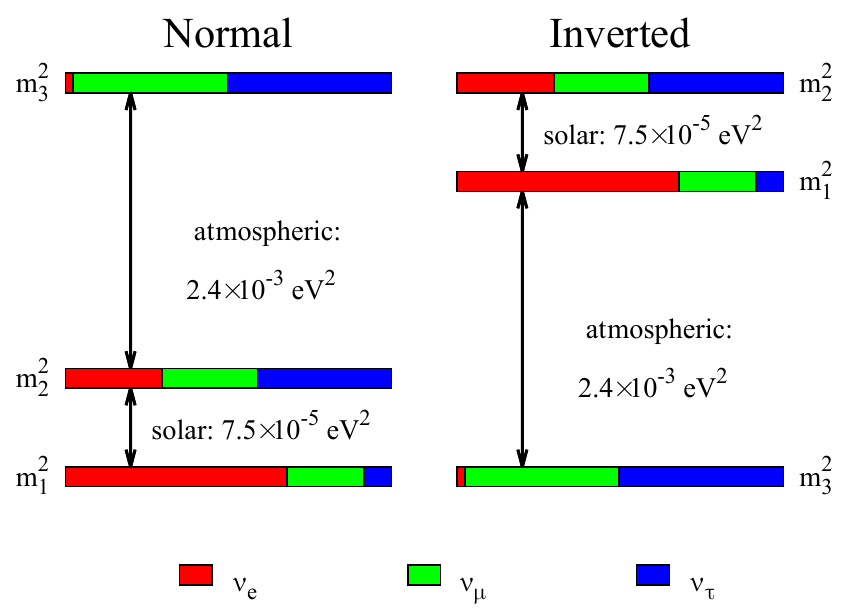
\includegraphics[scale=0.5]{massOrdering.png}
  \caption{The two possible \emph{mass hierarchies}, i.e., orderings of neutrino masses, as allowed by current data. From \cite{NuPhysWithJUNO}.}
  \label{fig:massOrdering}
\end{figure}

In an experiment like Daya Bay, where we are looking for the \emph{disappearance} of (anti)\-neu\-trinos of a given flavor, our interest is in \(P(\alpha \rightarrow \alpha)\). In this case, the behavior of neutrinos and antineutrinos is the same, and \eqref{eq:oscReIm} simplifies to
\begin{equation}
  P(\alpha \rightarrow \alpha) = 1 - 4 \sum_{j>i} |U_{\alpha j}|^2 |U_{\alpha
    i}|^2 \sin^2\left( \frac{\Delta m^2_{ji} L}{4E} \right). 
\end{equation}
The matrix elements from \eqref{eq:upmnsParam} can then be inserted in order to derive the disappearance probability for a particular flavor. For electron antineutrinos, as at Daya Bay, the survival probability is
\begin{align}
  \label{eq:survProbDybFull}
  \begin{split}
    P(\nubar_e \rightarrow \nubar_e) =
    1 &- \cos^4\theta_{13}\sin^2 2\theta_{12} \sin^2 \Delta_{21} \\
    &- \sin^2 2\theta_{13}\left( \cos^2\theta_{12} \sin^2 \Delta_{31} + \sin^2\theta_{12} \sin^2
      \Delta_{32}\right),
  \end{split}
\end{align}
where we've introduced the notation
\begin{align*}
  \Delta_{ji} &\equiv \frac{\Delta m^2_{ji}L}{4E}
           \approx \frac{1.267\, \Delta m^2_{ji}\,\mathrm{[eV^2]}\;
           L\,\mathrm{[m]}}{E\,\mathrm{[MeV]}}.
\end{align*}

Based on the value of $\Delta m^2_{21}$ given in \autoref{tab:pdgOscPars}, at the baselines of Daya Bay \(\sin^2 \Delta_{21}\) is so small that the experiment has no ability to constrain $\theta_{12}$ (nor \(\Delta m^2_{21}\) itself). In this analysis, then, $\theta_{12}$ and $\Delta m^2_{21}$ are fixed to the global values. This leaves $\theta_{13}$, \(\abs{\Delta m^2_{31}}\), and \(\abs{\Delta m^2_{32}}\). However, given that the difference between \(\abs{\Delta m^2_{31}}\) and \(|\Delta m^2_{32}|\) is less than one part in thirty, distinguishing between their corresponding phases would require some combination of a high-resolution detector and a baseline long enough to stretch out the phase difference. At Daya Bay, the baseline of $\sim$1~km is approximately one oscillation length, where the detector resolution is insufficient for resolving the difference. Therefore, Daya Bay cannot measure the two splittings jointly. On the other hand, since \(\Delta m^2_{21}\) is well constrained and known to be positive, we can tightly relate \(\abs{\Delta m^2_{31}}\) and \(\abs{\Delta m^2_{32}}\):
\begin{equation}
  \label{eq:hierarchy}
  \abs{\Delta m^2_{31}} =
  \begin{cases*}
    \abs{\Delta m^2_{32}} + \Delta m^2_{21}, & normal hierarchy ($\Delta m^2_{32} > 0$), \\
    \abs{\Delta m^2_{32}} - \Delta m^2_{21}, & inverted hierarchy ($\Delta m^2_{32} < 0$), \\
  \end{cases*}
\end{equation}
Thus, by using this relation to eliminate one parameter, it is possible to perform a two-parameter fit of \eqref{eq:survProbDybFull} directly, \emph{provided that the mass hierarchy is specified}. Since the mass hierarchy is currently unknown, two sets of results must be reported; furthermore, they are subject to change if an improved determination of \(\Delta m^2_{21}\) is ever published.

Alternatively, we can recast \eqref{eq:survProbDybFull} in a form that refers only to an empirical \emph{effective} mass splitting \(\Delta m^2_{ee}\):
\begin{equation}
  \label{eq:survProbDybEE}
  P(\nubar_e \rightarrow \nubar_e) \approx 1 - \cos^4\theta_{13}\sin^2 2\theta_{12} \sin^2 \Delta_{21}
  - \sin^2 2\theta_{13}\sin^2\Delta_{ee},
\end{equation}
where
\begin{equation}
  \Delta_{ee} \equiv \frac{\Delta m^2_{ee}L}{4E}. 
\end{equation}
It must be noted that \eqref{eq:survProbDybEE} is not an exact reparameterization of \eqref{eq:survProbDybFull}, since the former contains only two frequencies rather than three. Again, however, Daya Bay cannot resolve between $\Delta_{31}$ and $\Delta_{32}$, so there is no practical loss in sensitivity with this approach. The advantage of it is that it produces a single value that is independent of the mass hierarchy and immune to changes wrought by updates to \(\Delta m^2_{21}\).

\(\Delta m^2_{ee}\), as used here, has an \emph{operational,} rather than a physical, definition: It is simply the value that, when inserted into \eqref{eq:survProbDybEE}, gives the best fit to the data.
%
\begin{comment}
  Note that, if Daya Bay only measured antineutrinos at a single $L/E$, we could instead have made a truly physical definition of $\Delta m^2_{ee}$ by declaring that \[ \sin^2 \Delta_{ee} \equiv \cos^2\theta_{12} \sin^2 \Delta_{31} + \sin^2\theta_{12} \sin^2 \Delta_{32}. \] However, the righthand side of this definition depends on $L/E$, so unless this dependence is shown to be negligible, it cannot be used in broadband analyses such as Daya Bay's.
\end{comment}
%
In Daya Bay's case, however, \(\Delta m^2_{ee}\) can be related to physical quantities to a very good degree of approximation. Returning to \eqref{eq:survProbDybFull}, it can be shown \cite{DocDbDm2ee} that, in Daya Bay's range of $L/E$,
\begin{equation}
  \label{eq:dmPhi}
  \cos^2\theta_{12} \sin^2\Delta_{31} + \sin^2\theta_{12}\sin^2\Delta_{32}
  \approx \sin^2 (\Delta_{32} \pm \phi),
\end{equation}
where
\begin{equation}
  \phi \equiv \arctan\left( \frac{\sin2\Delta_{21}}{\cos2\Delta_{21}+ \tan^2
      \theta_{12}} \right),
\end{equation}
and ``+'' (``--'') corresponds to the normal (inverted) hierarchy. Inserting \eqref{eq:dmPhi} into \eqref{eq:survProbDybFull} and comparing to \eqref{eq:survProbDybEE} gives the approximate relation
\begin{equation}
  \label{eq:dmPhiApprox}
  \Delta m^2_{ee} \approx \abs{\Delta m^2_{32}} \pm \Delta m^2_\phi/2,
\end{equation}
where
\begin{equation}
  \Delta m^2_\phi = \frac{4\phi E}{L}.
\end{equation}
Although $\Delta m^2_\phi$ depends on $L/E$, for Daya Bay it is essentially constant and equal to \(\cos^2\theta_{12}\Delta m^2_{21}\). Inserting that into \eqref{eq:dmPhiApprox}, we find that, for both mass hierarchies,
\begin{equation}
  \label{eq:dmPhysical}
  \Delta m^2_{ee} \approx \abs{\Delta m^2_{31}\cos^2\theta_{12}} + \abs{\Delta m^2_{32}\sin^2\theta_{12}}.
\end{equation}
For all intents and purposes, this approximation is exact at Daya Bay. Hence Eqs. \eqref{eq:dmPhysical} and \eqref{eq:hierarchy} can be used to relate Daya Bay's measured \(\Delta m^2_{ee}\), as operationally defined by \eqref{eq:survProbDybEE}, to the physical mass splittings:
\begin{align*}
  \abs{\Delta m^2_{31}} = \Delta m^2_{ee} + \sin^2 \theta_{12} \Delta m^2_{21}, \qquad
  & \abs{\Delta m^2_{32}} = \Delta m^2_{ee} - \cos^2 \theta_{12} \Delta m^2_{21} \qquad
  & \text{(NH)}\\
  % 
  \abs{\Delta m^2_{31}} = \Delta m^2_{ee} - \sin^2 \theta_{12} \Delta m^2_{21}, \qquad
  & \abs{\Delta m^2_{32}} = \Delta m^2_{ee} + \cos^2 \theta_{12} \Delta m^2_{21} \qquad
  & \text{(IH)}
\end{align*}
Of course, in doing so, one must still specify the mass hierarchy and \(\Delta m^2_{21}.\) As a sanity check, Daya Bay has compared the results of fitting \eqref{eq:survProbDybFull} and \eqref{eq:survProbDybEE}, finding that, in the end, both techniques give the same values of \(\abs{\Delta m^2_{32}}\) and \(\abs{\Delta m^2_{31}}\). For the sake of simplicity, this analysis will use \eqref{eq:survProbDybEE} and fit \(\Delta m^2_{ee}\).

\section{History of neutrino oscillations}
\label{sec:history}

In the late 1960s, deep in the Homestake mine located in South Dakota, Ray Davis filled a large tank with tetrachloroethylene, a common dry-cleaning agent, and waited as solar neutrinos interacted with chlorine-37 atoms via the reaction
\begin{equation}
  \mathrm{\nu_e + \ ^{37}Cl \longrightarrow \ ^{37}Ar + e^-.}  
\end{equation}
Every few weeks, from 1970 to 1994, helium was bubbled through the liquid to extract the few dozen argon atoms that were produced in the time since the previous extraction. Each extraction was then placed in a gas-filled proportional chamber, where the $^{37}$Ar decays (roughly one per week) were counted over the course of a year or so (long enough to count effectively all of the atoms, given the 35-day half-life of $^{37}$Ar). By the early 1970s, the measurements were clearly indicating a reaction rate that was one-third of the prediction derived from the Standard Solar Model (SSM) \cite{DAVIS199413}. This ``solar neutrino problem'' was interpreted to mean that either the SSM or the experiment was in error, and neutrinos remained, according to the wisdom of the day, massless.

Despite the prevailing belief in masslessness, the possibility of massive neutrinos was considered as early as 1962, soon after the discovery that neutrinos come in separate electron and muon flavors. That year, in the ``MNS'' paper by Maki, Nakagawa, and Sakata \cite{10.1143/PTP.28.870}, the authors considered the possibility of neutrino flavor mixing, possibly from a nonzero mass. Neutrino mixing had been considered previously by Pontecorvo in 1957 \cite{Pontecorvo:1957cp}, but in the form of neutrino-antineutrino mixing, in analogy with the then-recently discovered phenomenon of neutral kaon mixing \cite{PhysRev.105.1925.2}. Pontecorvo revisited the subject in 1967, building upon the MNS formalism to describe how oscillations could occur in travelling neutrinos, going so far as to suggest that solar neutrinos could oscillate (well before the first experimental hints of such by the Davis experiment). Still, it would take decades of further obervations to prove that these four theorists were correct.

The late 1980s delivered additional anomalies, when the Kamiokande \cite{HIRATA1988416} and IMB \cite{PhysRevLett.66.2561} experiments observed a deficit in the number of atmospheric charged-current \(\mathrm{\nu_\mu}\) events relative to expectations. In addition, Kamiokande also confirmed the solar neutrino problem \cite{SUZUKI199554}, which was yet again confirmed around 1992 by the gallium-based SAGE \cite{GAVRIN200136} and GALLEX \cite{VIGNAUD199820} radiochemical experiments. In 1996, the massive Super-Kamiokande (SK) water Cerenkov detector came online, and in 1998 the SK collaboration published measurements of the zenith angle dependence of the atmospheric neutrino deficit \cite{PhysRevLett.81.1562}. This geometric dependence was consistent with mass-induced flavor oscillations. Other models, such as neutrino decay or decoherence, were disfavored by the SK data, which was of sufficient quality to provide initial values of \(\theta_{23}\) and \(\Delta m^2_{32}\) (defined in \autoref{sec:oscPhysics}). Super-Kamiokande's compelling evidence in favor of nonzero neutrino mass would soon receive confirmation from other experiments.

Such confirmation arrived dramatically in 2002, thanks to the Sudbury Neutrino Observatory (SNO) \cite{PhysRevLett.89.011301}. Owing to its use of heavy water as the target material, SNO had unprecedented sensitivity to neutral current (NC) interactions, which are undergone by all three neutrino flavors. This NC sensitivity stood in addition to SNO's customary sensitivity to charged current (CC) interactions, which (at the relevant energy scale of $\sim$10~MeV) only provide detection of electron neutrinos. As such, SNO was capable of independently measuring both the total and the electron neutrino fluxes. The total flux was in excellent agreement with the SSM, demonstrating that the ``missing'' neutrinos underlying the solar neutrino problem were, in fact, merely hiding in the form of muon and tau neutrinos. SNO thus succeeded both in confirming the existence of neutrino mass and in resolving the solar neutrino problem, once and for all.

At this point, the existence of neutrino oscillations was no longer a question, but a fact. The precision era had begun, and the Japan-based reactor neutrino experiment KamLAND was one effort that had gotten a head start. KamLAND was initially proposed to search for potential oscillation in 1994, when the solar measurements were still murky, but by 1997 there was enough evidence from the results of Davis, SAGE, and GALLEX to suggest that KamLAND might be able to measure $\theta_{12}$ and $\Delta m^2_{21}$, if indeed such parameters were responsible for the solar neutrino deficit (and assuming that $\theta_{12}$ was sufficiently large, which remained an open question). Around the time of SNO's announcement, KamLAND published results on the disappearance of reactor antineutrinos over long ($\sim$100~km) baselines \cite{PhysRevLett.90.021802}. KamLAND succeeded in pinning down the value of $\theta_{12}$, in favor of the large mixing angle solution, and furthermore provided what remains the most precise measurement of \(\Delta m^2_{21}\) ever performed.

Meanwhile, the atmospheric results of SK and others on \(\Delta m^2_{32}\) had set off a flurry of successful long-baseline accelerator experiments, such as K2K \cite{PhysRevD.74.072003}, T2K \cite{ABE2011106}, MINOS \cite{PhysRevLett.101.131802}, NO$\nu$A \cite{PhysRevLett.123.151803}, OPERA \cite{Agafonova_2012}, and ICARUS \cite{Rubbia_2011}, optimized for this mass splitting and designed to narrow down its value and that of $\theta_{23}$. As the 2010s approached, however, one mixing angle remained elusive: $\theta_{13}$.

The disappearance of electron (anti)neutrinos is controlled by $\theta_{12}$ and \(\Delta m^2_{21}\) at longer baselines (such as those employed in solar neutrino experiments and KamLAND) and by $\theta_{13}$ and \(\Delta m^2_{31}\) at shorter baselines. As luck would have it, at the energies of reactor antineutrinos, the latter oscillation length is $\sim$1~km, which is a sufficiently short distance that a relatively modest target mass of $\sim$10~tons will provide ample statistics from a typical commercial power reactor. By adopting such baselines and target masses, the Chooz experiment in France, as well as the Palo Verde experiment in the USA, set the stage for the reactor-based study of neutrino oscillations. Unfortunately, for Chooz and Palo Verde, sensitivity to oscillations was limited, in large part due to the dependence of a single-detector configuration on modeling the absolute reactor antineutrino flux.\footnote{Rapid deterioration of the gadolinium-doped scintillator was another obstacle.} These two experiments were unable to discover evidence of oscillation, instead setting upper limits of roughly $\sin^2 2\theta\,<\,0.17$ (for a mass-squared splitting of $|\Delta m^2_{32}| \approx 2.5\times10^{-3}\,\text{eV}^2$). Importantly, however, this result excluded $\nu_\mu \rightarrow \nu_e$ oscillations as the driver of the atmospheric $\nu_\mu$ disappearance seen by experiments such as Super-K.

In order to mitigate the uncertainty arising from modeling of the absolute antineutrino flux, the subsequent generation of reactor experiments were designed using identical detectors at different baselines \cite{Mikaelyan:1998yg}. This would enable the near detectors to measure the antineutrino flux while the far detectors measure any oscillation. Uncertainties on the absolute flux and detection efficiency thus largely cancel in the far/near ratio. The Double Chooz \cite{Ardellier:2006mn}, RENO \cite{Ahn:2010vy}, and Daya Bay \cite{Guo:2007ug} experiments embarked on this effort in parallel. This thesis describes, in detail, an analysis of Daya Bay's data in order to extract $\theta_{13}$ and the associated mass splitting.


\section{History of reactor neutrino experiments}
\label{sec:introReactor}

Although a number of reactor-based experiments were briefly described in \ref{sec:history}, the history of the field merits further discussion, given that this thesis is based on one such experiment. Nuclear reactors have played an important role in experimental neutrino physics since the very beginning. Indeed, the Savannah River reactor provided the antineutrinos that led to the first direct confirmation of the particle's existence by the 1956 Cowan-Reines experiment. Since then, reactors have continued to provide key insights into the nature of the neutrino.

Essentially all reactor neutrino experiments are based on detecting charged-current inverse beta decay (IBD) interactions in a volume of liquid scintillator, observed by photomultipler tubes. The details of this measurement principle are discussed in \autoref{chap:experim}. Among its advantages are (a) the fact that the double-pulse signature allows efficient background rejection without the need to evade cosmogenic backgrounds by going deep underground (especially important at km and shorter baselines, where a deep overburden would create challenging logistics), (b) the threshold energy is lower compared to a water Cerenkov detector, and (c) the materials and technology are inexpensive in comparison to advanced designs such as noble liquid time projection chambers. These advantages have remained pertinent from the Cowan-Reines experiment up to the present day.

Efforts involving reactor neutrinos gained steam in the 1970s, when interest arose in going beyond merely using nuclear reactors to qualitatively confirm the neutrino's existence and interactions. One of the new goals was to quantitatively measure the flux and spectrum of electron antineutrinos produced by nuclear reactors. These efforts bore fruit in the early-to-mid 1980s when a half-dozen experiments\footnote{ILL, Gosgen, Rovno, Krasnoyarks, Bugey, and Savannah River.} published such measurements \cite{PhysRevD.24.1097,Zacek:1986cu,Afonin:1985rw,Aleshin_2008,Abbes:1995nc,Sobel:1982gf}. These early detectors were relatively small, with target masses of a few hundred kg (versus Daya Bay's 80~t at the far site); hence, short baselines (of 10--100~m) were necessary in order to obtain sufficient statistics. The fluxes measured by these experiments were in good agreement with the predictions of the ILL-Vogel model \cite{SCHRECKENBACH1985325,VONFEILITZSCH1982162,HAHN1989365,PhysRevC.24.1543}, which was developed around the same time. Much later, as discussed in \autoref{chap:reactor}, these measurements would provide evidence of the so-called reactor antineutrino anomaly \cite{PhysRevD.83.073006} associated with the Huber-Mueller reevaluations of the predicted flux \cite{PhysRevC.84.024617,PhysRevC.83.054615}, which lie $\sim5$\% higher than the measured fluxes. In addition, the data from one of these experiments (Bugey-3) would later be combined with Daya Bay's in order to set limits on light sterile neutrino mixing \cite{PhysRevLett.117.151801}.

The 1990s brought the Chooz \cite{Apollonio_2003} and Palo Verde \cite{PhysRevD.64.112001} experiments (mentioned previously in the context of neutrino oscillations), which employed larger, $\mathcal{O}$(10~t) detectors so as to acquire useful statistics at longer (km-scale) baselines. Although the search for oscillations was their primary goal, these two experiments were also able to measure the $\nubar_e$ flux at these longer baselines, comparable to the average baseline for the Daya Bay far site. 
% \footnote{XXX When was it fully confirmed that $\nu_\mu \rightarrow \nu_\tau$ was the explanation, rather than $\nu_\mu \rightarrow \nu_s$?}
As with the short-baseline experiments, Chooz and Palo Verde would later indicate a $\sim5$\% deficit with respect to the Huber-Mueller flux predictions.

The $\theta_{13}$ sector is not the only one in which reactor antineutrinos can play a useful role. The KamLAND experiment used reactors to confirm and complement the solar neutrino results on $\theta_{12}$ and $\Delta m^2_{21}$, significantly improving the precision on the latter. Located a kilometer underground in Japan's Kamioka mine, in the cavern formerly occupied by the Kamiokande-II detector, KamLAND employed a massive, transparent balloon filled with 1000~t of liquid scintillator \cite{PhysRevLett.90.021802}. Antineutrinos arrived from some 50 reactors scattered throughout Japan, at a flux-averaged baseline of 180~km. This $L/E$ was well-suited for measuring oscillations driven by $\Delta m^2_{21}$, and KamLAND's measurement of this splitting will remain unchallenged for the foreseeable future.
% Unrelated to reactor neutrinos, KamLAND was also the first experiment to observe \emph{geoneutrinos} \cite{kamlandGeo}, that is, antineutrinos produced by the decay chains of $^{238}$U and $^{232}$Th in the Earth.

Returning to the topic of $\theta_{13}$, in 1998, Mikaelyan and Sinev \cite{Mikaelyan:1998yg} rigorously showed that a two-detector (near and far) reactor experiment could overcome the absolute flux uncertainty and allow for precision measurement of $\sin^2 2\theta_{13}$. Although beam experiments also carry the potential to measure $\theta_{13}$ by observing $\nu_\mu \to \nu_e$ oscillation, they are susceptible to degeneracies between it and other parameters, such as the mass hierarchy, $\dcp$, and the other mixing angles. Reactors thus remained a favorible means to a pure $\theta_{13}$ measurement, despite the fact that disappearance channels are generally more challenging than appearance channels when measuring a small mixing angle.

Accordingly, in the mid-2000s, the Double Chooz \cite{Ardellier:2006mn}, RENO \cite{Ahn:2010vy}, and Daya Bay \cite{Guo:2007ug} experiments were proposed. All three shared the same basic design: Near and far detectors at a $\mathcal{O}$(1 km) (far) baseline, using gadolinium-doped liquid scintillator to improve detection efficiency and background rejection. In April 2011, Double Chooz began taking far site data, followed in August by RENO's full configuration, and in December by Daya Bay using a six-detector configuration. In March 2012, with just 55 days of data, Daya Bay announced a $5.2\sigma$ discovery of nonzero $\theta_{13}$ \cite{PhysRevLett.108.171803}, which was quickly confirmed by RENO in the following weeks \cite{PhysRevLett.108.191802}. Since then, these experiments have continued to publish increasingly precise measurements of $\theta_{13}$ and $\Delta m^2_{ee}$, as well as measurements of the absolute flux (confirming the anomaly) \cite{PhysRevD.100.052004,Atif:2020eyo,DoubleChooz2020}, the spectrum (discovering an as-yet unexplained excess of events around 5~MeV, relative to predictions) \cite{PhysRevD.100.052004,Atif:2020eyo,DoubleChooz2020}, and, at least in the case of Daya Bay, the time evolution of the flux and spectrum \cite{PhysRevLett.118.251801}, the decomposed fuel isotope components of the flux and spectrum \cite{PhysRevLett.123.111801}, sterile neutrino limits \cite{PhysRevLett.117.151801}, decoherence limits \cite{DayaBayWavePacket}, and numerous other valuable results, demonstrating the major scientific utility of reactor neutrino experiments.

Recent years have seen a resurgence of activity in short-baseline ($\sim$5--25~m) reactor experiments, motivated both by the need for precise measurement of the reactor antineutrino flux/spectrum as well as by the prospect of an eV-scale sterile neutrino (as suggested, controversially, by the reactor antineutrino anomaly \cite{PhysRevD.83.073006}, the SAGE/GALLEX anomalies \cite{PhysRevC.80.015807,KAETHER201047}, and the anomalous $\nu_e$ results of the LSND and MiniBooNE accelerator experiments \cite{PhysRevD.64.112007,PhysRevLett.121.221801}). These ton-scale experiements\footnote{Among them, NEOS \cite{Ko:2019cip}, DANSS \cite{Alekseev_2016}, STEREO \cite{Allemandou_2018}, PROSPECT \cite{ASHENFELTER2019287}, NEUTRINO-4 \cite{Serebrov:2020kmd}, and SoLiD \cite{Abreu_2021}} complement each other with different reactor types (commercial or research), baselines/mobility, scintillator materials (liquid or plastic), neutron capture isotopes (Gd or $^6$Li), and levels of segmentation (3D, 2D, or none). With the exception of SoLiD, all of these experiments have already published valuable results, including new limits on sterile neutrino mixing around 1~eV$^2$ \cite{PhysRevLett.118.121802,Svirida:2019kbq,PhysRevD.102.052002,PhysRevD.103.032001}, strong rejection of sterile neutrinos as the explanation of the reactor antineutrino anomaly \cite{PhysRevD.102.052002,PhysRevD.103.032001}, confirmation of the 5~MeV bump \cite{PhysRevLett.118.121802}, and precise measurement of nearly-pure antineutrino spectra from $^{235}$U \cite{PhysRevD.103.032001}. Intriguingly, NEUTRINO-4 has claimed a $4.6\sigma$ discovery of sterile neutrino mixing at a $\Delta m^2$ of 7.25~eV$^2$ \cite{Serebrov_2020}, but time will tell whether this is borne out by other experiments.

Finally, looking to the future, the 20~kt JUNO detector \cite{juno} (in southern China) will be by far the largest reactor neutrino detector ever constructed. The driving goal of the JUNO experiment is the determination of the mass hierarchy (see \autoref{sec:majorana}) without susceptibility to the degeneracies and correlations that complicate the hierarchy determination in accelerator experiments \cite{Ghosh:2017sli}. JUNO will observe $\nubar_e$ interactions using more efficient PMTs and significantly larger photocathode coverage in order to achieve sub-3\% energy resolution. At this resolution, the two hierarchies produce measurable differences in the high-frequency oscillations due to $\theta_{13}$ of the $\nubar_e$ spectrum. If JUNO is successful, it could determine the mass hierarchy years before other (beam-based) experiments are expected to do so, cementing yet another historical achievement for the humble reactor antineutrino.

\subfilebackmatter

\end{document}
